\documentclass[11pt]{article}  % Sets the font size to 12 pt and document type to article

% =============================
% Essential Packages
% =============================
\usepackage[utf8]{inputenc}     % Ensures proper encoding of special characters
\usepackage[T1]{fontenc}        % Improved font encoding
\usepackage{amsmath, amsfonts, amssymb} % Common math packages
\usepackage{geometry}           % More intuitive control over margins
\usepackage{fancyhdr}           % Custom headers and footers
\usepackage{lmodern}            % Improved Latin Modern font
%\usepackage{setspace}          % Uncomment for line spacing adjustments (e.g., \doublespacing)
\usepackage[most]{tcolorbox}
\usepackage{enumitem} 
\usepackage{tikz}
\usetikzlibrary{positioning,shapes,arrows.meta,calc} % <-- added calc

\tikzset{
  block/.style={draw, rounded corners, minimum width=26mm, minimum height=7mm, align=center},
  norm/.style={draw, rounded corners, minimum width=20mm, minimum height=7mm, align=center},
  plus/.style={circle, draw, inner sep=0pt, minimum size=4mm},
}



% =============================
% Color Box
% =============================

\newtcolorbox{notebox}[2][]{%
  colback=yellow!10!white,
  colframe=yellow!50!black,
  coltitle=black,
  fonttitle=\normalfont,
  enhanced,
  attach boxed title to top left={yshift=-2mm,xshift=5mm},
  boxed title style={colback=yellow!50!white},
  title={#2},
  sharp corners=south,
  rounded corners=northwest,
  #1
}

% =============================
% Page Layout
% =============================
\geometry{
  left=1in,
  right=1in,
  top=1in,
  bottom=1in
}

% =============================
% Header Setup
% =============================
\pagestyle{fancy}
\fancyhf{}  % Clear default header/footer
\fancyhead[R]{\today}
\fancyhead[C]{Norm Selection}
\fancyhead[L]{}
\renewcommand{\headrulewidth}{0.4pt}  % Header line thickness


% =============================
% Macros
% =============================
\usepackage{url}            % simple URL typesetting
\usepackage{booktabs}       % professional-quality tables
\usepackage{amsfonts}       % blackboard math symbols
\usepackage{nicefrac}       % compact symbols for 1/2, etc.
\usepackage{microtype}      % microtypography
%\usepackage[table]{xcolor}         % colors
\usepackage{bbm}
%\usepackage{dsfont}
\usepackage{tcolorbox}
\usepackage{euscript}    %  
\usepackage{makecell}
\usepackage{times}
\RequirePackage{fix-cm}
\usepackage{cmap}                   %   PDF
\usepackage{comment}
\usepackage{xr}
\usepackage{tikz}
%\usepackage{extsizes} %   14- 
\usepackage{csquotes} %   
\usepackage{siunitx}
\usepackage{float}
\restylefloat{table}
\usepackage{array}
%\usepackage{undertilde}
\usepackage{setspace} % 
%\onehalfspacing %  1.5
%\doublespacing %  2
%\singlespacing %  1f
\usepackage[export]{adjustbox}
\usepackage{lastpage} % ,     .
\usepackage{soulutf8} %  
\usepackage{icomma} % "" : $0,2$ --- , $0, 2$ --- 
%\newenvironment{solution}
%{\renewcommand\qedsymbol{$\blacksquare$}\begin{proof}[Solution]}{\end{proof}}
\usepackage{diagbox, eqparbox, hhline}
\usepackage{etoolbox}
\usepackage{mathtools}
\usepackage{etextools}
\usepackage{ifthen}
\usepackage{caption}
\usepackage{subcaption}
\usepackage{amsmath,amssymb, amsthm}
%\usepackage{charter}
%\usepackage{calc}
\usepackage[flushleft]{threeparttable} % http://ctan.org/pkg/threeparttable
\usepackage{calligra}
\usepackage{layout}
\usepackage{lipsum}
%\mathtoolsset{showonlyrefs=true}
\usepackage{mathrsfs}
\usepackage{color}
\usepackage{setspace}
\usepackage{multicol} %  
\usepackage{filecontents}
%nwork with tables
\usepackage{array,tabularx,tabulary,booktabs} %    
%\usepackage{longtable}  %  
\usepackage{multirow} %    
\usepackage{graphicx}
%\usepackage{subfig}
\usepackage{fancyhdr}
\usepackage{theoremref}
\usepackage{pifont}%for defining \xmark
%\usepackage[noend]{algpseudocode}
%\usepackage{verbatim}
%\usepackage[ruled,vlined]{algorithm2e}

\usepackage{algorithm}
\usepackage{algpseudocode}

\usepackage[colorinlistoftodos,bordercolor=orange,backgroundcolor=orange!20,linecolor=orange,textsize=scriptsize]{todonotes}
\usepackage{xspace}

\usepackage{hyperref}       % hyperlinks
\usepackage{cleveref}

\usepackage{enumitem}


\usepackage{wrapfig}
\usepackage{listings}
\usepackage{xcolor}
\lstdefinestyle{mystyle}{
    language=Python,
    basicstyle=\ttfamily\small,
    keywordstyle=\color{blue},
    stringstyle=\color{red},
    commentstyle=\color{gray},
    numbers=left,
    numberstyle=\tiny,
    stepnumber=1,
    breaklines=true,
    tabsize=4
}



\lstset{style=mystyle}


%%%%%%%%%%%%%%
%NEW COMMANDS   %%%
%%%%%%%%%%%%%%
\DeclareMathOperator*{\prox}{prox}
\DeclareMathOperator*{\brox}{brox}
\DeclareMathOperator*{\argmax}{arg\,max}
\DeclareMathOperator*{\argmin}{arg\,min}
\DeclareMathOperator*{\sign}{sign}
\DeclareMathOperator*{\sgn}{sgn}
\DeclarePairedDelimiter\abs{\lvert}{\rvert}

\newcommand{\inner}[2]{\left\langle #1, #2 \right\rangle}

% macros.tex

\newcommand{\mA}{\mathbf{A}}
\newcommand{\mB}{\mathbf{B}}
\newcommand{\mC}{\mathbf{C}}
\newcommand{\mD}{\mathbf{D}}
\newcommand{\mE}{\mathbf{E}}
\newcommand{\mF}{\mathbf{F}}
\newcommand{\mG}{\mathbf{G}}
\newcommand{\mH}{\mathbf{H}}
\newcommand{\mI}{\mathbf{I}}
\newcommand{\mJ}{\mathbf{J}}
\newcommand{\mK}{\mathbf{K}}
\newcommand{\mL}{\mathbf{L}}
\newcommand{\mM}{\mathbf{M}}
\newcommand{\mN}{\mathbf{N}}
\newcommand{\mO}{\mathbf{O}}
\newcommand{\mP}{\mathbf{P}}
\newcommand{\mQ}{\mathbf{Q}}
\newcommand{\mR}{\mathbf{R}}
\newcommand{\mS}{\mathbf{S}}
\newcommand{\mT}{\mathbf{T}}
\newcommand{\mU}{\mathbf{U}}
\newcommand{\mV}{\mathbf{V}}
\newcommand{\mW}{\mathbf{W}}
\newcommand{\mX}{\mathbf{X}}
\newcommand{\mY}{\mathbf{Y}}
\newcommand{\mZ}{\mathbf{Z}}

\newcommand{\ma}{\mathbf{a}}
\newcommand{\mb}{\mathbf{b}}
\newcommand{\mc}{\mathbf{c}}
\newcommand{\md}{\mathbf{d}}
\newcommand{\me}{\mathbf{e}}
\newcommand{\mf}{\mathbf{f}}
\newcommand{\mg}{\mathbf{g}}
\newcommand{\mh}{\mathbf{h}}
\newcommand{\mi}{\mathbf{i}}
\newcommand{\mj}{\mathbf{j}}
\newcommand{\mk}{\mathbf{k}}
\newcommand{\ml}{\mathbf{l}}
\newcommand{\mm}{\mathbf{m}}
\newcommand{\mn}{\mathbf{n}}
\newcommand{\mo}{\mathbf{o}}
\newcommand{\mpp}{\mathbf{p}}
\newcommand{\mq}{\mathbf{q}}
\newcommand{\mr}{\mathbf{r}}
\newcommand{\ms}{\mathbf{s}}
\newcommand{\mt}{\mathbf{t}}
\newcommand{\muu}{\mathbf{u}}
\newcommand{\mv}{\mathbf{v}}
\newcommand{\mw}{\mathbf{w}}
\newcommand{\mx}{\mathbf{x}}
\newcommand{\my}{\mathbf{y}}
\newcommand{\mz}{\mathbf{z}}


% Calligraphic letters
\newcommand{\cA}{\mathcal{A}}
\newcommand{\cB}{\mathcal{B}}
\newcommand{\cC}{\mathcal{C}}
\newcommand{\cD}{\mathcal{D}}
\newcommand{\cE}{\mathcal{E}}
\newcommand{\cF}{\mathcal{F}}
\newcommand{\cG}{\mathcal{G}}
\newcommand{\cH}{\mathcal{H}}
\newcommand{\cI}{\mathcal{I}}
\newcommand{\cJ}{\mathcal{J}}
\newcommand{\cK}{\mathcal{K}}
\newcommand{\cL}{\mathcal{L}}
\newcommand{\cM}{\mathcal{M}}
\newcommand{\cN}{\mathcal{N}}
\newcommand{\cO}{\mathcal{O}}
\newcommand{\cP}{\mathcal{P}}
\newcommand{\cQ}{\mathcal{Q}}
\newcommand{\cR}{\mathcal{R}}
\newcommand{\cS}{\mathcal{S}}
\newcommand{\cT}{\mathcal{T}}
\newcommand{\cU}{\mathcal{U}}
\newcommand{\cV}{\mathcal{V}}
\newcommand{\cW}{\mathcal{W}}
\newcommand{\cX}{\mathcal{X}}
\newcommand{\cY}{\mathcal{Y}}
\newcommand{\cZ}{\mathcal{Z}}

% Bracket macros
\newcommand{\cbrac}[1]{\left\{ #1 \right\}}   % Curly braces
\newcommand{\sbrac}[1]{\left[ #1 \right]}     % Square brackets
\newcommand{\rbrac}[1]{\left( #1 \right)}     % Round parentheses
% Norm macro
\newcommand{\norm}[1]{\left\lVert #1 \right\rVert}
\newcommand{\normsub}[2]{\left\lVert #1 \right\rVert_{#2}}
\newcommand{\normarrow}[3]{\left\lVert #1 \right\rVert_{#2 \rightarrow #3}}
\newcommand{\normabs}[1]{\left\lvert #1 \right\rvert}


\let\la=\langle
\let\ra=\rangle

\def\<{\left\langle}
\def\>{\right\rangle}
% \def\[{\left[}
%\def\]{\right]}
\def\({\left(}
\def\){\right)}

%\newcommand{\st}{\;:\;}
\newcommand{\ve}[2]{\langle #1 ,  #2 \rangle}

%\newcommand{\eqdef}{\stackrel{\text{def}}{=}}
\newcommand{\eqdef}{:=}
\newcommand{\ii}{{}^{(i)}}


\newcommand{\Prob}{\mathbf{Prob}}
\newcommand{\E}{\mathbf{E}}
\newcommand{\R}{\mathbb{R}}
\newcommand{\N}{\mathbb{N}}


% sets
\DeclareMathOperator{\card}{card}       % cardinality of a set
\DeclareMathOperator{\diam}{diam}       % diameter of a set
\DeclareMathOperator{\MVEE}{MVEE}       % minim volume enclosing ellipsoid of a set
\DeclareMathOperator{\vol}{vol}         % volume of a set

% statistical
% \DeclareMathOperator{\Exp}{{\rm E}}           % expectation
%\newcommand{\Exp}[1]{{\rm E}\left[#1\right]}
\newcommand{\Exp}[1]{\mathbb{E}\left[#1\right]}
\newcommand{\Expu}[2]{\mathbb{E}_{#1}\left[#2\right]}
\newcommand{\ExpSub}[2]{\mathbb{E}_{#1}\left[#2\right]}
% Trace macro
\newcommand{\tr}[1]{\mathrm{tr}\left(#1\right)}


\DeclareMathOperator{\Cov}{Cov}         % covariance
\DeclareMathOperator{\Var}{Var}         % variance
\DeclareMathOperator{\Corr}{Corr}       % correlation
\DeclareMathOperator{\LMO}{LMO} 

% functions and operators
\DeclareMathOperator{\signum}{sign}     % signum/sign of a scalar
\DeclareMathOperator{\dom}{dom}         % domain
\DeclareMathOperator{\epi}{epi}         % epigraph
\DeclareMathOperator{\Ker}{null}        % nullspace/kernel
\DeclareMathOperator{\nullspace}{null}  % nullpsace
\DeclareMathOperator{\range}{range}     % range
\DeclareMathOperator{\Image}{Im}        % image

% topology
\DeclareMathOperator{\interior}{int}    % interior
\DeclareMathOperator{\ri}{rint}         % relative interior
\DeclareMathOperator{\rint}{rint}       % relative interior
\DeclareMathOperator{\bdry}{bdry}       % boundary
\DeclareMathOperator{\cl}{cl}           % closure

% vectors, matrices
\DeclareMathOperator{\linspan}{span}
\DeclareMathOperator{\linspace}{linspace}
\DeclareMathOperator{\cone}{cone}

%\DeclareMathOperator{\tr}{tr}           % trace
\DeclareMathOperator{\rank}{rank}       % rank
\DeclareMathOperator{\conv}{conv}       % convex hull
\DeclareMathOperator{\Diag}{Diag}       % Diag(v) = diagonal matrix with v_i on the diagonal
\DeclareMathOperator{\diag}{diag}       % diag(D) = the diagonal vector of matrix D

\DeclareMathOperator{\Arg}{Arg}         % Argument




\newtheorem{theorem}{Theorem}
\newtheorem{proposition}{Proposition}

\theoremstyle{plain}

\newtheorem{example}{Example}
\newtheorem{assumption}{Assumption}
\newtheorem{lemma}{Lemma}
\newtheorem{fact}{Fact}

\newtheorem{prop}[theorem]{Proposition}
\newtheorem{corollary}{Corollary}
\newtheorem{lem}[theorem]{Lemma}
\newtheorem{claim}[theorem]{Claim}
\newtheorem{remark}{Remark}


\newtheorem{exercise}[theorem]{Exercise}

\newtheorem{rem}[theorem]{Remark}
\newtheorem{que}[theorem]{Question}
\newtheorem{definition}{Definition}


%zerosarah paper symbols

\newcommand*{\qedb}{\hfill\ensuremath{\square}}   % or \blacksquare
\newcommand{\topic}[1]{\vspace{2mm}\noindent{{\bf #1:}}}
\newcommand{\head}[1]{\noindent{{\bf #1:}}}

\definecolor{mydarkgreen}{RGB}{39,130,67}
\definecolor{mydarkred}{RGB}{192,47,25}
\definecolor{mydarkblue}{RGB}{39,47,180}
\definecolor{mydarkpurple}{RGB}{48,25,52}
\newcommand{\green}{\color{mydarkgreen}}
\newcommand{\red}{\color{mydarkred}}
\newcommand{\blue}{\color{mydarkblue}}
\newcommand{\purple}{\color{mydarkpurple}}

\newcommand{\zerosarah}{{\sf ZeroSARAH}\xspace}
\newcommand{\clip}{\operatorname{clip}}



\definecolor{lightblue}{RGB}{224, 240, 255} % Adjust RGB values as needed
\definecolor{bgcolor}{rgb}{0.8,1,1}
\definecolor{bgcolor2}{rgb}{0.8,1,0.8}
\newenvironment{proofof}[1]{\smallskip\noindent{\bf \em Proof of #1.}}%





\newcommand{\peter}[1]{\todo[inline]{\textbf{Peter: }#1}}
\newcommand{\igor}[1]{\todo[inline]{\textbf{Igor: }#1}}
\newcommand{\abdurakhmon}[1]{\todo[inline]{\textbf{Abdurakhmon: }#1}}
\newcommand{\hanmin}[1]{\todo[inline]{\textbf{Hanmin: }#1}}

\newcommand{\algname}[1]{{\sf \footnotesize \color{mydarkgreen} #1}\xspace}

%\newcommand{\theHalgorithm}{\arabic{algorithm}}


\newcommand{\rA}{{\red A}}
\newcommand{\rB}{{\red B}}

\newcommand{\dmodel}{d_{\text{model}}}
\newcommand{\dhead}{d_{\text{head}}}
\newcommand{\RBLDh}{\R^{B \times L \times \dhead}}
\newcommand{\RBLDm}{\R^{B \times L \times \dmodel}}
\newcommand{\RBLE}{\R^{B \times L \times E}}
\newcommand{\softmax}{\text{softmax}}
\newcommand{\floor}[1]{\left\lfloor #1 \right\rfloor}
\newcommand{\boxtext}[1]{\boxed{\text{#1}}}
\newcommand{\prob}[1]{\mathbb{P}\rbrac{#1}}
\newcommand{\probsub}[2]{\mathbb{P}_{#1}\rbrac{#2}}
\newcommand{\din}{d_{\text{in}}}
\newcommand{\dout}{d_{\text{out}}}
\newcommand{\klD}[2]{{\rm D}_{\text{KL}}\rbrac{#1 \parallel #2}}
\newcommand{\pisub}[3]{\pi_{#1}\rbrac{#2 \mid #3}}
\newcommand{\thetaold}{\theta_{\text{old}}}
\newcommand{\thetaref}{\theta_{\text{ref}}}  % No .tex extension needed


% =============================
% Begin Document
% =============================
\begin{document}

\section{Linear Algebra}


\subsection{Column wise decomposition.}
Any matrix $\mA \in \R^{m \times n}$ can be decomposed into the sum of its columns: 
\begin{align}
	\mA = \sum_{i=1}^{n} \mA_{:j} e_j^{\top},
\end{align}
where $e_j$ are standard basis vectors of $\R^n$.
Notice that this is a rank $1$ decomposition.

\subsection{Row wise decomposition.}
Any matrix $\mA \in \R^{m \times n}$ can be decomposed into the sum of its rows: 
\begin{align}
	\mA = \sum_{i=1}^{m} e_i \mA_{i:}^{\top},
\end{align}
where $e_i$ are standard basis vectors of $\R^m$.
Notice that this is a rank $1$ decomposition.


\section{LLM Training}
\subsection{Scaling the logits after LLM head.}
We usually apply RMS norm to normalize (along the last dimension $E$, where it stands for model dimension, $B$ means batch size and $L$ means sequence length) the tensor $\mX \in \R^{B \times L \times E}$ we feed into LLM head, and obtain the corresponding logits $l$.
After RMS normalization, each tensor corresponding to the token $x_i \in \R^E$ will then have ${\rm RMS}(x_t) = 1$.
Now notice that for each coordinate $x_{i, t}, t\in[E]$, treating as a random variable, its variance is given by 
\begin{align}
  \Var\rbrac{x_{i, t}} = \Exp{x^2_{i, t}} - \rbrac{\Exp{x_{i, t}}}^2,
\end{align}
and if it is zero-mean (or small), then $\Var\rbrac{x_{i, t}} \simeq \Exp{x^2_{i, t}}$, which is to say that second moment reflects the variance.

The next step is to use the empirical observation that for linear layers, hidden vectors tend to be approximatedly rotation-invariant (isotropic), i.e., each coordinate behaves like the others, so we can use the second moment over the coordinate in a token to replace the actual second moment.
And the former, is given by 
\begin{align}
  \Var\rbrac{x_{i, t}} \simeq \frac{1}{E}\sum_{t=1}^{E}x_{i, t} = 1.
\end{align}
Now we start to consider the logits, which is generated by 
\begin{align*}
  l_{j, i} = w_j^{\top}x_i = \sum_{t=1}^{E}w_{j, t}x_{i, t}.
\end{align*}
If we assume each weight entry $w_{j, t}$ are i.i.d. with variance $\sigma^2$ the logits variance is give by 
\begin{align*}
  \Var\rbrac{l_{j, i}} = \sum_{t=1}^{E} \sigma^2 \Var \rbrac{x_{t, i}} \simeq E \sigma^2.
\end{align*}
So the standard deviation $\sim \sqrt{E}$.
To ensure that logits do not scale with the model dimension, we scale it by $\sqrt{E}$.



\section{Attention}

\subsection{Multihead Self Attention (MHA)}
Consider an input tensor $\mX \in \R^{B \times L \times d_{\text{model}}}$ to an attention layer, where $B$ is the batch size, $L$ is the sequence length, and $d_{\text{model}}$ is the model dimension.

\begin{enumerate}
  \item The first step involves computing queries, keys, and values. 
  We have three matrices, $\mW_q$, $\mW_k$, and $\mW_v \in \R^{d_{\text{model}} \times d_{\text{model}}}$, and simultaneously perform the following operations
  \begin{align}
    \mQ = \mX \mW_{q};\quad \mK = \mX \mW_{k};\quad \mV = \mX\mW_{v}.
  \end{align}
  These operations are vectorized, meaning that for each sequence $b$ in the batch of size B, we do 
  \begin{align*}
    \mQ_b = \mX_b\mW_{q} \quad \forall b \in [B].
  \end{align*} 
  $\mW_q$, $\mW_k$, and $\mW_v$ are trainable parameters shared across the entire batch. 
  The resulting $\mQ$, $\mK$, and $\mV$ have the shape $\R^{B \times L \times d_{\text{model}}}$.

  \item Next, for multihead attention, we reshape $\mQ$, $\mK$, and $\mV$ from shape $\R^{B \times L \times d_{\text{model}}}$ into $\R^{B \times H \times L \times d_{\text{head}}}$, where $H$ is the number of attention heads and $d_{\text{head}}$ is the dimension of each head.
  To achieve this, we first divide $d_{\text{model}}$ into $H$ heads, resulting in shapes of $\R^{B \times L \times H \times d_{\text{head}}}$. 
  Then we rearrange into $\R^{B \times H \times L \times d_{\text{head}}}$.
  Conceptually, each head uses a subset of dimensions from $d_{\text{model}}$ to compute scores between queries and keys along the sequence dimension $L$.
  We will use the following notations $\mQ_h, \mK_h, \mV_h$ to denote the per head tensor in $R^{B \times 1 \times L \times d_{\text{head}}}$ for each head $h \in [H]$.

  \item In the next step, we perform the attention calculation:
  \begin{align*}
    \mS_h &\eqdef \text{Scores}_h(\mQ_h, \mK_h) = \frac{\mQ_h \mK_h^{\top}}{\sqrt{d_{\text{head}}}} + \mM\\
    \mA_h &\eqdef \text{Attention}_h(\mQ, \mK, \mV) = \text{softmax}\rbrac{\mS_h}\mV_h, \quad \forall h \in [H].
  \end{align*}
  The scaled multiplication of $\mQ_h$ and $\mK^{\top}_h$ is vectorized, resulting in $\mS_h \in \R^{B\times 1\times L \times L}$ and $\mS \in \R^{B\times H\times L \times L}$.\footnote{Here $\mS$ is the stack of $\mS_h$ along dimension $H$.}
  Optionally, we could use a mask matrix to mask out certain tokens, an example would be the causual self attention.
  To stabilize the gradients, we element-wise divide raw scores by $\sqrt{d_{\text{head}}}$.
  This scaling choice can be justified because each element of $\mQ_h\mK_h^{\top}$ represents a dot product between vectors of dimension $d_{\text{model}}$. 
  The variance of this dot product scales as $\Var\rbrac{\inner{q_h}{k_h}}\sim d_{\text{model}}\sigma_q^2\sigma_k^2$. 
  Since variance scales quadratically, we divide by $\sqrt{d_{\text{head}}}$.
  The softmax operation turns the scores after masking into probabilities, along the last dimension.\footnote{This is to say that for each $L \times L$ matrix, we softmax every row.}
  Imagine $z = [z_1, \hdots, z_L] \in \R^L$ is a row vector, then essentially, softmax defines the operation:
  \begin{align}
    \sigma(z)_i \eqdef \frac{e^{z_i}}{\sum_{j=1}^{L}e^{z_j}}.
  \end{align}
  Sometimes we use a numerically stable version to replace it 
  \begin{align}
    \tilde{\sigma}(z) \eqdef \frac{e^{z_i - \max(z)}}{\sum_{j=1}^{L}e^{z_j - \max(z)}}.
  \end{align}

  It is worth mentioning that in single head attention (scaled dot product), the complexity of computation is $\cO\rbrac{BL^2d_{\text{model}}}$, while for multihead attention, it is the same since we do $\cO\rbrac{H \times BL^2d_{\text{head}}} = \cO\rbrac{BL^2d_{\text{model}}}$. 

  \item Finally, we concatenate and mix attention outputs from all heads. 
  Concatenation involves first transposing $\mA_h$ to $\R^{B \times L \times H \times d_{\text{head}}}$ and then merging the last two dimensions into $\mA \in \R^{B \times L \times d_{\text{model}}}$. 
  This concatenated result is projected using a matrix $\mW_O$, as follows:
  \begin{align}
    \text{MHA}(\mX) = \mA\mW_{O}. 
  \end{align}
  The final output retains the shape $\R^{B \times L \times d_{\text{model}}}$.
\end{enumerate}
There a bunch of reasons why we are using multi heads instead of scaled dot product attention. 
\begin{itemize}
  \item \textbf{Diversity of learned attention patterns}: Each head learns different attention patterns in parallel. 
  A single attention head computes only one set of attention scores.

  \item \textbf{Subspace specialization}: Instead of operating in $d_{\text{model}}$, each head projects to a lower dimension subspace $d_{\text{head}}$.
  This suggests that each head operates in a distinct feature subspace.

  \item \textbf{Improved gradient flow and representation mixing}: Independent paths improve gradient flow and richness of learned representations.
\end{itemize}
Notice that the compuatational cost are the \textbf{SAME}!

\subsection{Multi Query Attention (MQA)}
In MQA, different heads have its own query, but share the same key and value.
Specifically, for a head $h$, we have 
\begin{align*}
  \mS_h &\eqdef \text{Scores}(\mQ_h, \mK) = \frac{\mQ_h\mK^{\top}}{\sqrt{d_{\text{head}}}} + \mM \\
  \mA_h &\eqdef \text{Attention}_h (\mQ_h, \mK, \mV) = \text{softmax}(\mS_h)\mV, \quad \forall h \in [H]. 
\end{align*}
This means that for each head $h$, we have a separate $\mQ_h \in \R^{B \times 1 \times L \times d_{\text{head}}}$ and shared $\mK, \mV \in \R^{B \times 1 \times L \times d_{\text{head}}}$.

Compared to standrad MHA, MQA has the following features:
\begin{itemize}
  \item \textbf{Reduced parameter count}: Each head has its own query only, shared key and value.
  \item \textbf{Smaller activation size (memory usage)}: Now $\mK, \mV \in \R^{B \times 1 \times L \times d_{\text{head}}}$, so the activation size is smaller.
  \item \textbf{Reduced KV cache (fast inferencing)}: For transformer based models such as GPT, we generate text one token at a time. 
  To avoid recomputing attention over all previous tokens on every step, we cache $k, v$ (key and value vectors) for all previously seen tokens.
  Specifically, in standard MHA, for each layer and token generated, we neeed $2BHLd_{\text{head}}$ for cached $\mK, \mV$.
  In MQA, we share $\mK$ and $\mV$ so that the cost becomes $2BLd_{\text{head}}$.
  \item \textbf{Minimal accuracy loss.} Used in GPT-3.5, PaLM, LLaMA, etc.
\end{itemize}

\subsection{KV cache}
The motivation for KV caching is to enable efficient inference — both in terms of compute time and memory bandwidth.
At inference time only, autoregressive models input a sequence of tokens $\cbrac{x_t, \hdots, x_{t + L - 1}}$ to generate the next token $x_{t + L}$. 
To avoid recomputing key and value vectors for all previous tokens every time, we cache the $k, v$ pairs corresponding to the tokens $x_t \hdots, x_{t + L - 1}$ in the forward pass.
Then, when generating $x_{t + L + 1}$, we can reuse the vectors for cached $x_{t + 1}, \hdots, x_{t + L - 1}$ and we only need to compute $k, v$ for $x_{t + L}$. 
This mechanism is known as the \textbf{KV cache}.


\subsection{Grouped Query Attention (GQA)}
GQA is like an interpolation between MQA and MHA, where we ask groups of heads to share $\mK, \mV$.
Specifically, let $g(h)$ be a function that maps a head $h$ to its corrsponding group index, then we have 
\begin{align*}
  \mS_h &\eqdef \text{Scores}(\mQ_h, \mK_{g(h)}) = \frac{\mQ_h\mK^{\top}_{g(h)}}{\sqrt{d_{\text{head}}}} + \mM \\
  \mA_h &\eqdef \text{Attention}_h (\mQ_h, \mK_{g(h)}, \mV_{g(h)}) = \text{softmax}(\mS_h)\mV_{g(h)}, \quad \forall h \in [H]. 
\end{align*} 
Benefits:
\begin{enumerate}
  \item Less memory than MHA.
  \item Flexible compute/memory tradeoff by controlling the number of k, v heads.
\end{enumerate}
It is used in LLaMA 2 and Mistral.



\subsection{Multihead Latent Attention (MLA)}
Before we go into details, we need to first differentiate between self attention and cross attention. 
\begin{itemize}
  \item Self attention is the case when Q, K, V comes from the same input sequence. Its typically used in encoder blocks of BERT, GPT, LLaMA, etc, and decoder blocks in GPT, T5, etc.
  \item Cross attention refers to the case when Q comes from one sequence but K, V comes from another sequence. It is typically used in the case that decoder attends to encoder outputs (T5, BART), and the case of vision language models where text attends to image, and perceiver-style latent attention.
\end{itemize}
We can formulate cross attention in the following way: Let $\mZ \in \R^{B \times M \times d_{\text{model}}}$ (expanded from $\R^{1 \times M \times d_{\text{model}}}$.) be a target sequence (queries) and $\mX \in \R^{B \times L \times d_{\text{model}}}$ be a source sequence (keys and values),
\begin{align}
  \mQ = \mZ\mW_q; \quad \mK = \mX\mW_k; \quad \mV = \mX\mW_v.
\end{align}
Notice that $M$ could be different than $L$.
In the case of cross-attention with a latent array, we often have, $M << L$, which significantly reduces computational cost by avoiding full self-attention over the entire input sequence.
We then compute the attention scores and softmax:
\begin{align}
  \mS_h &\eqdef \text{Scores}(\mQ_h, \mK_{h}) = \frac{\mQ_h\mK^{\top}_{h}}{\sqrt{d_{\text{head}}}} \\
  \mA_h &\eqdef \text{Attention}_h (\mQ_h, \mK_{h}, \mV_{h}) = \text{softmax}(\mS_h)\mV_{h}, \quad \forall h \in [H].
\end{align}
Notice that in this case $\mS_h \in \R^{B \times 1 \times M \times L}$ and $\mA_h \in \R^{B \times 1 \times M \times d_{\text{head}}}$ for head $h \in [H]$. 
After concatenation, we result in $\mA \in \R^{B, M \times d_{\text{model}}}$, which is like we are focusing on a smaller sequence.
In MLA, latent vector it self is a learnable parameter and shared accross a batch. 
These latents act like information bottleneck that extract useful features from the long input $\mX \in \R^{B \times L \times d_{\text{model}}}$.



\subsection{Latent Transformer Block}
This is a key design of Perceiver (2021, DeepMind), Set Transformer and efficient transformers for long inputs (e.g., audio, video, documents).
Essentially it can be viewed as cross attention followed by latent self-attention.
Mathematically speaking, we are giving a vector $\mX \in \R^{B \times L \times d_{\text{model}}}$. 
First we are using the latent vector $\mZ \in \R^{1 \times M \times d_{\text{model}}}$ (expanded accross batch dimension.) and the input $\mX \in \R^{B \times L \times d_{\text{model}}}$, we have 
\begin{align*}
  \mA_1 = \text{Attention}(\mX_q = \mZ, \mX_k = \mX, \mX_v = \mX),
\end{align*}
which essentially asks "What should I learn from all of you tokens?".
After this step: each latent now contains information extracted from the input.
Notice that now $\mA_1 \in \R^{B \times M \times d_{\text{model}}}$ is a compressed representation of $\mX$, extracted by the latent array.
Then we do normal self attention on the latent variable:
\begin{align*}
  \mA_2 = \text{Attention}(\mX_q = \mA_1, \mX_k = \mA_1, \mX_v = \mA_1)
\end{align*}
where each latent vector is allowed to look at other latents, share what they learned and refine itself.
\begin{verbatim}
  for each block:
    z = z + CrossAttention(q ← z, k ← x, v ← x)
    z = z + SelfAttention(q ← z, k ← z, v ← z)    
\end{verbatim}
Before we actually feed the $\mZ$ and $\mX$ into the attention block and the final feed forward layer, we first do normlization (LayerNorm in the case of my code).



\subsection{Pre- and Post- Normlization}
In general, there are two ways of doing layer normlization, Post-LN and Pre-LN. 
In the original implementation of transformer, post-LN is used. 
However, pre-LN has become the modern default, which is used in GPT-2/3/4, T5, LLaMA, PaLM, Perceiver, etc.
The benefits of using pre-LN includes the follows:
\begin{itemize}
  \item {\bf (Help gradient flow \& increasing training stability)}: In a deep stack, residual paths carry the untouched signal forward. 
  With Pre-LN, those residual paths also carry unit-variance, zero-mean activations (because they are already normalized). 
  That keeps gradients well-scaled and prevents the exploding / vanishing issues that appeared when stacking 24 - 100+ layers with Post-LN.
  Empirically, Pre-LN lets you train hundreds (even thousands) of layers with a stable learning rate schedule, whereas Post-LN often needed warm-up tricks or gradient clipping.
  \item {\bf (Easier optimization of very long sequences)}: Cross-entropy loss is applied after the final LayerNorm.
  With Post-LN every sub-layer's output is renormalized, the network must constantly “undo” those shifts.
  Pre-LN leaves the residual branch untouched, so the model can accumulate information across time steps or tokens without repeatedly rescaling it.
  \item {\bf (Faster convergence)}: Many ablations show ~ 1.3 - 1.5x faster convergence for GPT/T5 style models when switching from Post-LN → Pre-LN. This is because every tensor that flows straight down the stack (both forward activations and backward gradients through the residual skip) has mean 0 and variance 1, which helps stabilize second-moment estimate quickly for Adam.
  \item {\bf (Safer with half-precision / mixed-precision)}: Normalizing before the high-variance matrix multiplications keeps activations in a narrower numeric range, reducing overflow/underflow risk in FP16/BF16 training.
\end{itemize}


\textbf{LayerNorm:} Mathematically speaking, consider an input $\mX$ in the space $\R^{B \times L \times d_{\text{model}}}$, for the $l$-th token in the $b$-th batch
\begin{align*}
  \mL[b, l, :] = \text{LayerNorm}(\mX[b, l, :]) = \gamma \cdot \frac{X[b, l, :] - \mu_{n, l}}{\sqrt{\sigma^2_{b, l}} + \epsilon} + \beta, 
\end{align*}
where 
\begin{align*}
  \mu_{b, l} = \frac{1}{d_{\text{model}}}\sum_{i=1}^{d_{\text{model}}}\mX[b, l, i], \quad \sigma^2_{b, l} = \frac{1}{d_{\text{model}}}\sum_{i=1}^{d_{\text{model}}}\rbrac{\mX[b, l, i] - \mu_{b, l}}^2,
\end{align*}
$\gamma, \beta \in \R^{d_{\text{model}}}$ are learned shift and scale vectors.
Notice that statistics are computed per sample, per position, no batch coupling, so the network behaves the same in training and inference and is robust to batch-size 1. 
Its benefits includes: 
\begin{itemize}
  \item {\bf (Zero-mean, unit-var features).} Keeps dot-products in a predictable range, resulting in stable softmax gradients.
  \item {\bf (Identical behaviour in training / inferencing).} Important for autoregressive generation where batch size changes.
  \item {\bf (Works with any sequence length).} No running-average statistics needed.
\end{itemize}
In a simpler form, layernorm can be written as 
\begin{align*}
  \mL = \gamma \odot \frac{\mX - \mu}{\sqrt{\sigma + \epsilon}} + \beta,
\end{align*}
where all operations are elementwise.
Notice that $\gamma, \beta \in \R^{d_{\text{model}}}$ are learnable parameters.


\subsection{Dropout}
\paragraph{During Training:}
This refers to During training we randomly set a fraction of the sub-layer output activations to zero and scale the survivors.
Specifically, for $\mX \in \R^{B \times L \times d_{\text{model}}}$ and the drop out rate $0 < p < 1$, we sample a binary traning mask $\mM \in \cbrac{0, 1}^{B \times L \times d_{\text{model}}}$, using the Bernoulli($q$) distribution where $q = 1 - p$, we then apply 
\begin{align*}
  \widehat{\mX} = \frac{1}{q}\mX \odot \mM.
\end{align*}
$q$ is referred to as the keep probability, and we are trying to make $\Exp{\widehat{\mX}} = \mX$.
\paragraph{During Inferencing:}
At inference time the mask is removed and $\mX$ passes through unchanged.

Code: 
\begin{verbatim}
  torch.nn.Dropout(p=p)
\end{verbatim}

\subsection{DCA}
This one seems to be less well known, on medical image tasks.

\subsection{Linear Attention}

\subsection{Sparse Attention}


\section{Normalizations}
Besides the layer norm mentioned in the previous chapter, there are other norms used quite often.

\subsection{BatchNorm}
Batch norm is rarely used in language modeling especially in modern architectures. 
It is not sequence or position aware, and it requires consistent statistics over a batch, with variable-length sequences in language modeling, the batch statistics can be unstable and unreliable.
Furthermore, it mixes information from each sequences, but ideally we want to keep it separate. 
However, it is great for vision tasks

Mathematically, given an input $\mX \in \R^{B \times d}$, for each feature $j$, we have 
\begin{align*}
  \mu_j = \frac{1}{B}\sum_{i=1}^{B}\mX[i, j], \quad \sigma^2_j = \frac{1}{B}\sum_{i=1}^{B}(\mX[i, j] - \mu_j)^2.
\end{align*}
Then each value is normlized in a way that 
\begin{align*}
  \hat{X}[i, j] = \gamma[j] \frac{X[i, j] - \mu_j}{\sqrt{\sigma_j^2 + \epsilon}} + \beta[j],
\end{align*}
where $\gamma, \beta \in \R^d$ are learnable parameters per feature / channel.

If we are given an input 2D/Convolutional data $\mX \in \R^{B \times C \times H \times W}$, we have 
\begin{align*}
  \mu_c = \frac{1}{BHW}\sum_{b,h,w}\mX[b, c, h, w], \quad \sigma_c^2 = \frac{1}{BHW}\sum_{b,h,w}(\mX[b, c, h, w] - \mu_c)^2,
\end{align*}
basically, we are computing mean and variance per channel.
Notice that \textbf{LayerNorm is still the default in most Vision Transformer (ViT-style) backbones}. 
In CNN, sometimes GroupNorm replaces BatchNorm because it's batch-size independent and mixes well with vision features.


\subsection{RMSNorm}
Its name is Root Mean Square Layer Normalization, which has become popular in some recent LLMs, especially as a lighter and sometimes more numerically stable alternative to LayerNorm.
It normalizes only by root mean square of the features\footnote{Features in this context refer to the elements in dimension $d_{\text{model}}$} instead of mean and variance.
Given $X \in \R^{B \times L \times d_{\text{model}}}$ 
\begin{align*}
  \text{RMS}_{b, l} = \sqrt{\frac{1}{d_{\text{model}}}\sum_{i=1}^{d_{\text{model}}} \mX[b, l, i]^2 + \epsilon}
\end{align*}
Then, each element in $\mX$ is normalized by 
\begin{align*}
  \hat{X}[b, l, i] = \frac{\mX[b, l, i]}{\text{RMS}_{b, l}} \cdot \gamma_i, \qquad \forall i \in [d],
\end{align*}
where $\gamma_i$ is the $i$-th component of the learnable scaling factor $\gamma \in \R^{d_{\text{model}}}$.

LLaMA (and most of Meta-Llama 1/2/3 checkpoints) swap the original LayerNorm for pre-norm RMSNorm.

Below is a complete list of RMSNorm's features.
\begin{itemize}
  \item {\bf (Rescales by RMS only \& scaling only)}.
  \item {\bf (Compute \& Memory efficiency)}. ~ 30 \% cheaper per norm op; overall 2-6 \% faster end-to-end in large LLMs.
  \item {\bf (Numerically stable)}. Works well with very deep pre-norm Transformers.
\end{itemize}
When does it shine: (1) Ultra-deep LLMs, (2) Inference-first or edge deployments, (3) Pre-norm architectures.

RMSNorm really does skip the “subtract-the-mean” step, so a single normalization needs one less reduction-operation and a bit less memory traffic (removing the mean saves one vector reduction, one broadcast, and one add.). 
This skip would not affect training stability, because pre-norm residuals absorb the offset: in modern transformers RMSNorm sits before each residual branch, any mean shift can be compensated by the next linear layer's bias.
To see this: consider the following procedure, (assuming $x \in \R^d$)
\begin{align*}
  \boxed{x} \xrightarrow{\text{RMSNorm}} \boxed{y = \gamma \cdot \frac{x}{\norm{x}_{\text{RMS}}}} \xrightarrow{\mW, b} \boxed{u = \mW y + b} \xrightarrow{} \boxed{z = x + u}
\end{align*}
$y$ indeed does not have mean zero, denote it as $\mu_{y}$, since the next operation is affine, we can rewrite it as 
\begin{align*}
  u = \mW(y - \mu_{y}{\bf{1}}) + (b + \mW\mu_{y}{\bf{1}}),
\end{align*}
which means that it is equivalent to adjusting the bias. 
During training, back-prop will simply nudge $b$ so the network learns whatever overall shift is optimal, it does not care where that shift originates.
After that $u$ is added to the original $x$, but the drift in $\mu_{y}$ will not accumulate unchecked because: (1) The residual path still carries the original, unshifted activations, (2) The next block starts with another RMSNorm, which rescales its input (including any offset) back to a controlled RMS before new computations begin.



\section{Positional Embedding}




\section{Precisions}
Here is a summary provided by Chat-GPT o3.
% ---------------- Table 1: high / mid precision ----------------
\begin{table}[ht]
\centering
\renewcommand{\arraystretch}{1.15}
\begin{tabular}{@{}lccccc@{}}
\toprule
\textbf{Format} & \textbf{Bits} & \textbf{Exp/Mant} &
\textbf{Dynamic range$^\dagger$} & \textbf{ULP@1} &
\textbf{Typical use} \\
\midrule
FP32        & 32 & 8/23 & $1.2\!\times\!10^{-38}$-$3.4\!\times\!10^{38}$ & $2^{-23}$ & Master weights, optimiser \\
FP16 (IEEE) & 16 & 5/10 & $6.1\!\times\!10^{-5}$-$6.6\!\times\!10^{4}$   & $2^{-10}$ & Fwd/Bwd on Volta \& T4 \\
\textbf{bfloat16} & 16 & 8/7  & $1.2\!\times\!10^{-38}$-$3.4\!\times\!10^{38}$ & $2^{-7}$  & Default on A100/H100, TPU \\
TF32$^{*}$  & 19 & 8/10 & $\phantom{0}$same as FP32 & $2^{-10}$ & GEMMs on Ampere \\
\bottomrule
\end{tabular}
\caption{Mid-/high-precision dtypes widely used during LLM training.%
$^\dagger$Smallest positive \emph{normal} value to largest finite.%
$^{*}$TF32 is a compute mode; tensors stored as FP32.}
\end{table}

% ---------------- Table 2: low precision & INT -----------------
\begin{table}[ht]
\centering
\renewcommand{\arraystretch}{1.15}
\begin{tabular}{@{}lccccc@{}}
\toprule
\textbf{Format} & \textbf{Bits} & \textbf{Exp/Mant} &
\textbf{Dynamic range$^\dagger$} & \textbf{ULP@1} &
\textbf{Typical use} \\
\midrule
FP8-E4M3 & 8 & 4/3 & $9.2\!\times\!10^{-8}$-$4.5\!\times\!10^{2}$  & $2^{-3}$ & Research train / fast inf.\ (H100) \\
FP8-E5M2 & 8 & 5/2 & $3.0\!\times\!10^{-10}$-$5.7\!\times\!10^{4}$ & $2^{-2}$ & Wider range variant (H100) \\
INT8 / INT4 & 8/4 & — & $\pm127$ / $\pm7$ & 1 / $1/16$ & Post-training inference quant. \\
\bottomrule
\end{tabular}
\caption{Very low-precision formats used for efficient training research (FP8) or deployment quantisation (INT).}
\end{table}

A floating point number in IEEE-style formats is stored as:
\begin{verbatim}
  Sign bit | Exponent bits | Mantissa (fraction) bits
\end{verbatim}
\begin{enumerate}
  \item \textbf{Sign bit}: ($1$ bit), $0$ positive and $1$ negative.
  \item \textbf{Exponent bits}: control the scale (powers of $2$). 
  More exponent bits means wider dynamic range.
  \item \textbf{Mantissa bits}: control the precision (how many distinct numbers you can represent between powers of 2). More mantissa bits means smaller ULP\footnote{Unit in the Last Place: The smallest possible difference between two representable floating-point numbers around a given value} (more precise).
\end{enumerate}
A number is typically constructed in this way:
\begin{align*}
  (-1)^{\text{sign}} \times (1.\text{mantissa bits}) \times 2^{\text{exponent} - \text{bias}}.
\end{align*}

\begin{itemize}
  \item \textbf{FP32} is used as the safe baseline in deep learning, it is almost always used for the master weigts\footnote{Master weight refers to the full-precision copy of the model's parameter that we keep during mixed-precision training.} and optimizer state because it is numerically stable.
  
  \item \textbf{FP16} is used in forward/backward pass to save memory in Volta(Nvidia V100)/T4 mixed-precision training. Prone to overflow/underflow unless scaled (hence loss scaling).
  
  \item \textbf{Loss scaling} refers to the practice we multiply our loss by a large constant $S$ before back propagation: $L_{\text{scaled}} = S \cdot L$, this scales up gradients which avoids gradient underflow. 
  However, after computing the gradients, we divide them by $S$ before updating the weights to restore correct magnitude. 
  NVIDIA's AMP (Automatic Mixed Precision) does dynamic loss scaling, adjusting $S$ automatically to prevent overflow. 

  \item \textbf{bfloat16} is Brain floating point came from Google Brain, whose exp bits are same as \textbf{FP32}, but the mantissa bits are much fewer, this avoids the over/under-flow problem in \textbf{BF16}. 
  This comes at a price of lower precision, but it is the default choice on A100 and H100.

  FP16 on Volta/T4 is fast but fragile, and requires loss scaling, which is why bfloat16 became popular. 
  It enjoys the same range as FP32, but no scaling headaches.

  Its advantage includes: (i) no losss scaling needed to handle with over/under flow, (ii) half the memory of \textbf{FP32}, (iii) speed up in matmul on A100/H100, (iv) can used as a drop in for \textbf{FP32}, because the dynamic range is the same.

  For downsides: (a) precisiob loss, (b) optimizers often still keep master weights in \textbf{FP32} to avoid cumulative rounding error, (c) numerically sensitive operations such as $\text{softmax}$/ normalization, kernel still uses \textbf{FP32} internally.

  \item \textbf{TF32}: NVIDIA introduced with Ampere GPUs (A100, RTX 3000 series), default in cuBLAS/cuDNN matmul on Ampere if you pass FP32 inputs. FP32's size and range, FP16's precision.
  
  \item \textbf{FP8-E4M3, FP8-E5M2}: We can now tell directly from their names that FP8-E4M3 has a narrower dynamic range at a higher precision. For FP8-E4M3, ULP@1 is $\frac{1}{2^3} = 0.125$ and for FP8-E5M2, the ULP@1 becomes $\frac{1}{2^2} = 0.25$ which is very coarse.
  
  E4M3: good for weights and activations that stay within a moderate range.

  E5M2: good for gradients or loss-related values that can swing wildly in magnitude.
\end{itemize}

\paragraph{How they (FP8) are used on H100:} It can be applied both for training and inferencing.

During \textbf{training:}
\begin{enumerate}
  \item Keep master weights in FP32 (like with FP16/bfloat16 training).
  \item Cast activations/gradients to FP8 for GEMMs inside the forward/backward pass.
  \item Apply per-tensor or per-channel \textbf{scaling} to map values into FP8's limited range.
  \item Often mix E4M3 for forward activations, E5M2 for backward gradients.
\end{enumerate}

During \textbf{Inferencing:}
Post-training quantization to FP8 for ultra-fast inference with minimal memory footprint.

\paragraph{Scaling is not optional:} FP8's numeric range is so tiny that, without actively scaling tensors before casting to FP8, we'll either hit overflow or underflow constantly.
The fix is that we multiply the tensor by a scaling factor S before FP8 conversion,
\begin{align*}
  x_{\text{scaled}} = x \times S.
\end{align*}
We may choose $S$ so that $\max{x_{\text{scaled}} }$ fits nicely into FP8's max normal value, and we store $S$ as a separate FP32 number. We can later undo the the scaling after computation:
\begin{align*}
  y = y_{\text{scaled}} \times S^{-1}.
\end{align*}
This keeps numbers inside FP8's safe zone while still preserving the original magnitude relationship.

\paragraph{Per channel vs. per tensor:}
Often, there are \textbf{per channel} scaling and \textbf{per tensor} scaling. Let us image that we are doing a fully-connected layer, where we have this weight matrix $\mW \in \R^{d_{\text{out}} \times d_{\text{in}}}$.
Per channel scaling means that we have a scaling factor for each output feature (each row), so there will be $d_{\text{out}}$ scalars, while for per tensor scaling, we only have $1$ scaling factor. In this sense, per tensor scaling is simpler, but will be suboptimal is some channels are loud and the others are quiet, while per channel scaling has better precisions, especially in convolutional layers or transformers where variance differs accross each head / filter.

\paragraph{Automation on H100:} Notice that there is automated scaling on NVIDIA H100, which tracks running max values for each tensor, and picks E4M3 (more precision) for forward activations, E5M2 (more range) for backward gradients.
The engine applies scaling transparently, so we mostly see FP8 without manually tuning the scaling factor $S$.
 
As an example of scaling, let us consider the previous example of fully connected layer, where we are expected to do $\mO = \mW\mX$, originally, both $\mW$ and $\mX$ are FP32 (master weights and full precision activations). 
Before GEMM\footnote{GEneral Matrix-Matrix Multiplication, in the form of $\mD = \alpha\cdot\mA\mB + \beta\mC$, where $\alpha, \beta$ are scalars. This is the workhorse of modern deep learning.}, we independently scaled them to FP8 (to fit the range) by 
\begin{align*}
  \mX_{\text{scaled}} = \mX \cdot S_{\mX}; \qquad \mW_{\text{scaled}} = \mW \cdot S_{\mW},
\end{align*}
then we performed the matmul in FP8, 
\begin{align*}
  \mO_{\text{scaled}} = \text{FP8GEMM}(\mW_{\text{scaled}}, \mX_{\text{scaled}}).
\end{align*}
To restore the original magnitude, we take advantage of the scaling factor $S_{\mX}, S_{\mW}$ who are FP32,
\begin{align*}
  \mO = \mO_{\text{scaled}} \cdot \frac{1}{S_{\mX}S_{\mW}}.
\end{align*}





\section{Encoder and Decoder Structure}

\paragraph{Encoder}
Typically, encodes looks like:

\begin{figure}[ht]
\centering

% ---------------- Pre-LN ----------------
\begin{minipage}{0.45\textwidth}
\centering
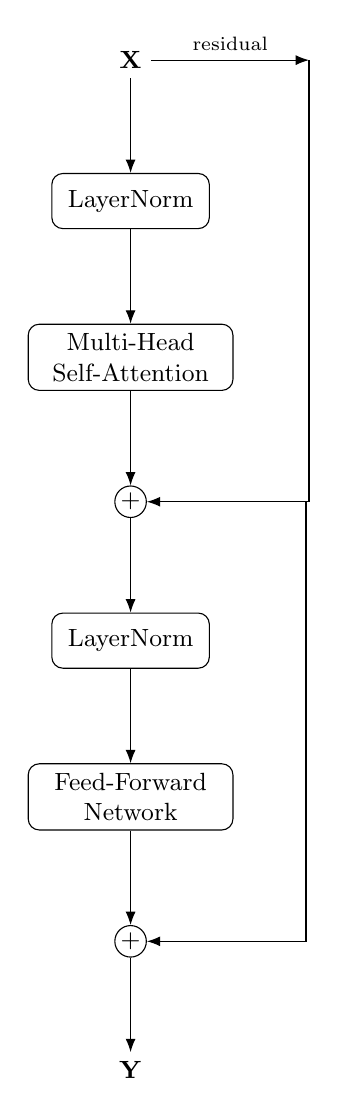
\begin{tikzpicture}[>=Latex, node distance=12mm, font=\small]
\node (x)   {$\mX$};
\node (ln0) [norm, below=of x] {LayerNorm};
\node (msa) [block, below=of ln0] {Multi-Head\\Self-Attention};
\node (add1)[plus,  below=of msa] {\small $+$};
\node (ln1) [norm,  below=of add1] {LayerNorm};
\node (ffn) [block, below=of ln1] {Feed-Forward\\Network};
\node (add2)[plus,  below=of ffn] {\small $+$};
\node (y)   [below=of add2] {$\mY$};

% main path
\draw[->] (x) -- (ln0);
\draw[->] (ln0) -- (msa);
\draw[->] (msa) -- (add1);
\draw[->] (add1) -- (ln1);
\draw[->] (ln1) -- (ffn);
\draw[->] (ffn) -- (add2);
\draw[->] (add2) -- (y);

% residuals
\coordinate (res1start) at ($(x.east)+(20mm,0)$);
\draw[->] (x.east) -- (res1start) node[midway,above] {\scriptsize residual};
\draw[->] (res1start) |- ($(add1.east)+(20mm,0)$) -- (add1.east);

\coordinate (res2start) at ($(add1.east)+(20.2mm,0)$);
\draw[->] (res2start) |- (add2.east);
\end{tikzpicture}

\small Pre-LayerNorm Transformer block
\end{minipage}%
\hfill
% ---------------- Post-LN ----------------
\begin{minipage}{0.45\textwidth}
\centering
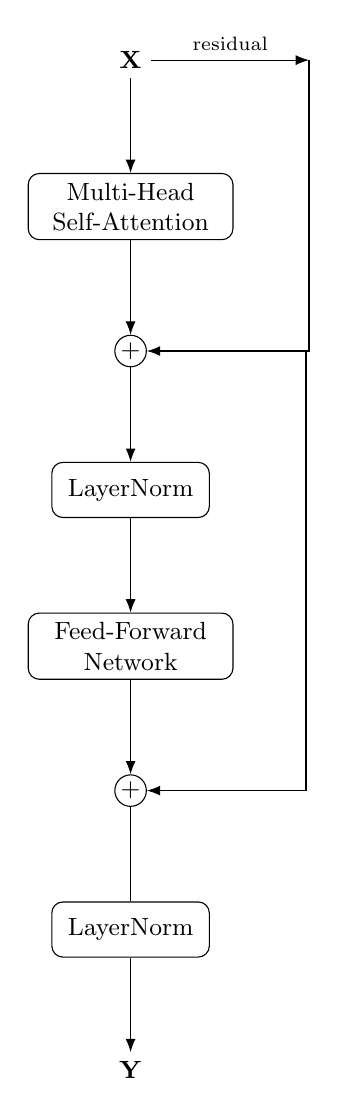
\begin{tikzpicture}[>=Latex, node distance=12mm, font=\small]
\node (x)   {$\mX$};
\node (msa) [block, below=of x] {Multi-Head\\Self-Attention};
\node (add1)[plus,  below=of msa] {\small $+$};
\node (ln1) [norm,  below=of add1] {LayerNorm};
\node (ffn) [block, below=of ln1] {Feed-Forward\\Network};
\node (add2)[plus,  below=of ffn] {\small $+$};
\node (ln2) [norm,  below=of add2] {LayerNorm};
\node (y)   [below=of ln2] {$\mY$};

% main path
\draw[->] (x) -- (msa);
\draw[->] (msa) -- (add1);
\draw[->] (add1) -- (ln1);
\draw[->] (ln1) -- (ffn);
\draw[->] (ffn) -- (add2);
\draw[->] (add2) -- (ln2) -- (y);

% residuals
\coordinate (res1start) at ($(x.east)+(20mm,0)$);
\draw[->] (x.east) -- (res1start) node[midway,above] {\scriptsize residual};
\draw[->] (res1start) |- ($(add1.east)+(20mm,0)$) -- (add1.east);

\coordinate (res2start) at ($(add1.east)+(20.2mm,0)$);
\draw[->] (res2start) |- (add2.east);
\end{tikzpicture}

\small Post-LayerNorm Transformer block
\end{minipage}

\end{figure}
As we have discussed before, the Pre-LayerNorm fashion is the current state of the art as its training is more stable, as well as its convergence. 
It helps gradient flow, and deep model stability, does not requries learning rate warm up and works better with long context.
It do has downside though, Pre-LN has a weaker normalizing effect so sometimes people add an extra final LayerNorm after the last layer for output stability (``final LN'' in GPT models).

\paragraph{Decoder}
\tikzset{
  block/.style={draw, rounded corners, minimum width=30mm, minimum height=7mm, align=center},
  norm/.style={draw, rounded corners, minimum width=22mm, minimum height=7mm, align=center},
  plus/.style={circle, draw, inner sep=0pt, minimum size=4mm},
}


\begin{figure}[ht]

\centering
\begin{tikzpicture}[>=Latex, node distance=12mm, font=\small]

% --- main vertical path (Pre-LN) ---
\node (x)   {$\mX$}; % decoder input (token embeddings or previous layer output)
\node (ln0) [norm,  below=of x]   {LayerNorm};
\node (msa) [block, below=of ln0] {Masked Multi-Head\\Self-Attention};
\node (add1)[plus,  below=of msa] {\small $+$};

\node (ln1) [norm,  below=of add1] {LayerNorm};
\node (csa) [block, below=of ln1] {Multi-Head\\Cross-Attention};
\node (add2)[plus,  below=of csa] {\small $+$};

\node (ln2) [norm,  below=of add2] {LayerNorm};
\node (ffn) [block, below=of ln2] {Feed-Forward\\Network};
\node (add3)[plus,  below=of ffn] {\small $+$};
\node (y)   [below=of add3] {$y$}; % decoder output

% --- encoder memory feeding cross-attention ---
% M: encoder hidden states, shape [T_enc x d_model]
\node (memtitle) [left=34mm of csa, align=left] {Encoder memory $\mM$\\ \footnotesize $\mM \in \mathbb{R}^{L_{\text{enc}}\times d_{\text{model}}}$};
% K,V label
\node (kvlabel) [below=1mm of memtitle, anchor=north west, align=left] {\footnotesize $\mK=\mW_{\mK} \mM,\;\;\mV=\mW_V \mM$};
\draw[->] (memtitle.east) -- (csa.west) node[midway,above] {\scriptsize $\mK,\mV$};

% --- main downward arrows ---
\draw[->] (x) -- (ln0) -- (msa) -- (add1) -- (ln1) -- (csa) -- (add2) -- (ln2) -- (ffn) -- (add3) -- (y);

% --- causal mask annotation into MSA ---

\node (masknote) [right=14mm of msa, align=left] {\scriptsize causal mask \\[-1pt] \scriptsize};
\draw[-{Latex}] (masknote.west) -- ++(-4mm,0) |- (msa.east);

% Optional: label MSA inputs as Q,K,V from LN(x)
\node (qkvmsa) [left=8mm of msa, align=right] {\scriptsize $\mQ,\mK,\mV$ \\ \scriptsize from $\mathrm{LN}(\mX)$};
\draw[-{Latex}] (qkvmsa.east) -- (msa.west);


% --- residuals aligned on a right column ---
\coordinate (rcol) at ($(x.east)+(23.3mm,0)$); % common right column for loops

% residual from x to add1 with explicit origin arrow
\draw[->] (x.east) -- (rcol) node[midway,above] {\scriptsize Residual};
\draw[->] (rcol) |- (add1.east);

% residual from after add1 to add2
\draw[->] ($(add1.east)+(24mm,0)$) |- (add2.east);

% residual from after add2 to add3
\draw[->] ($(add2.east)+(24mm,0)$) |- (add3.east);

\end{tikzpicture}

\caption{Pre-LN Transformer \textbf{Decoder} block. Each sublayer consumes a LayerNormed input. The masked self-attention applies a \emph{causal mask} (no future tokens). Cross-attention queries come from the decoder stream, while keys/values are derived from the encoder memory $\mM$ (encoder hidden states: $\mK=\mW_\mK\mM$, $\mV=\mW_\mV\mM$).}
\end{figure}

As a further explanation besides the figure: this $\mM$ is the matrix of encoder hidden states produced by the last encoder layer. It is what the decoder attends to in cross attention.
Let us image that an input $\mX \in \R^{B \times L_{\text{enc}} \times d_{\text{model}}}$ is fed into the encoder blocks. 
After embedding and positional encoding, we have 
\begin{align*}
  \mH^0 \in \R^{B \times L_{\text{enc}} \times d_{\text{model}}}.
\end{align*}
Each encoder will do 
\begin{align*}
  \mH^{k+1} = \text{Encoder}(\mH^k) \in \R^{B \times L_{\text{enc}} \times d_{\text{model}}}, \quad \forall k \in [N_{\text{enc}}],
\end{align*}
And $\mM$ is exactly $\mM = \mH^{N_{\text{enc}}}$.
As a result, for the cross attention layer: $\mK, \mV \in \R^{B \times L_{\text{enc}} \times d_{\text{model}}}$ and $\mQ \in \R^{B \times L_{\text{dec}} \times d_{\text{model}}}$, so the output of decoder block will always be $\R^{B \times L_{\text{dec}} \times d_{\text{model}}}$.

The two types of blocks are different:
\begin{itemize}
  \item Encoder: Self attention only, no masking, aiming to build a contextual representation of the entire source sequence.
  
  \item Decoder: Masked self attention, which prevents seeing future tokens so that the generation is autoregressive. 
  Cross attention, which lets each target position attend to the encoder's output $\mM$ (source context)
  The purpose overall is to generate the target sequence one step at a time, with access to both past target tokens and the entire source sequence.
\end{itemize}

What happens if we are using one type?
\begin{itemize}
  \item Encoder: leaking future target tokens during training (no causal mask), so the model wouldn't learn autoregressive generation.
  \item Decoder: useless masked self-attention in the encoder that blocks half the context for no reason, waste compute on a cross-attention sublayer when no encoder memory exists yet.
\end{itemize}

\paragraph{The original seq2seq transformer:} Things happens in two phases, 
\begin{verbatim}
Source tokens ---> [Encoder stack] ----------------> M (memory)
                                         |   
                                         v
Shifted target tokens ------> [Decoder stack] ---> Output logits
\end{verbatim}
Encoder runs once on the full source, decoder runs once (training) or incrementally (inference), always starting with shifted target embeddings as its own input stream.
The input of encoder is the source sequence $x = [x_1, x_2, ..., x_{L_{\text{enc}}}]$, after embedding we get $\mX$, while the input of the decoder is the target sequence $y$ so far, but shifted ($\hat{y}$) so that the model predicts the next token.
\begin{enumerate}
  \item We take the original gold target sequence $y = [y_1, y_2, ..., y_{L_{\text{dec}}}]$.
  \item Shift right by one and add the <BOS> special token, and obtain $\hat{y} = [<BOS>, y_1, ..., y_{L_{\text{dec}} - 1}]$, we then embed to get $\hat{\mY}$ ans use it as an input to the decoder blocks.
\end{enumerate}

\subsection{Encoder only models} 
BERT, RoBERTa, DeBERTa, ELECTRA, Sentence-BERT (SBERT). 

The architecture mostly are: \textbullet~ Stacks of encoder blocks only, \textbullet~ Full self attention, \textbullet~ Input sequence length stay fixed, \textbullet~ output contextualized embeddings for every token.

Purpose: Understand text: classification, regression, retrieval, token-level labeling (NER, POS tagging, QA span prediction). In those cases the model needs bidirectional context: token sees both left and right neighbors.

For many NLP tasks, we already have the full text and just need to analyze it, not generate it.

Advantages:
\begin{itemize}
  \item \textbf{Better context capture:} every token attends to all others.
  \item \textbf{More efficient training} for non-generative tasks (no need to autoregress).
  \item \textbf{Easier fine-tuning} for classification tasks: just take the [CLS] embedding\footnote{In BERT and similar models, we prepend a special token [CLS] (“classification”) to the start of every input sequence before feeding it to the encoder. [CLS] has its own trainable embedding vector in the model's vocabulary, just like any word. It is treated as position $0$ in the sequence and goes through all encoder layers along with the other tokens. After the final encoder layer, [CLS] has a contextualized vector $h \in \R^{d_{\text{model}}}$, which encodes information from the entire sequence (thanks to self-attention).}.
\end{itemize}

\subsection{Decoder only models}

GPT family (GPT-2, GPT-3, GPT-4, LLaMA, Mistral, Falcon, etc.); BLOOM, OPT, Pythia; Code generation models (CodeLLaMA, StarCoder)

Architecture: \textbullet~ Stack of decoder blocks only \textbullet~ Causal self-attention (mask future positions) \textbullet~ \textbf{No cross-attention} \textbullet~ Input length = current sequence length during generation.

Purpose: Generate text: language modeling, code generation; model learns 
\begin{align*}
  P(\text{next token} \mid \text{prev tokens})
\end{align*}

Advantages:
\begin{itemize}
  \item \textbf{Simpler}: do not need an encoder, since we aim to predict the next token given the past. Same architecture works for both pretraining (predict next token) and inference (sample next token)
  \item \textbf{Massive scalability}: can ingest any text corpus, no need for aligned parallel data.
  \item \textbf{Flexible prompts}: can condition on arbitrary text in-context.
\end{itemize}

\subsection{Encoder-decoder models}
often on seq2seq task, requires paired data\footnote{An example is that machine translation needs paired data: Source: "I like apples", Target: "J'aime les pommes".}.

As a summary:
\begin{table}[h]
\centering
\renewcommand{\arraystretch}{1.2}
\begin{tabular}{|l|p{5cm}|p{5cm}|}
\hline
\textbf{Model type} & \textbf{Pros} & \textbf{Cons} \\
\hline
\textbf{Encoder-only} & 
\textbullet~ Strong understanding with bidirectional context 

\textbullet~Great for classification, retrieval, and embedding learning
& 
\textbullet~ Not suited for generative tasks \\
\hline
\textbf{Decoder-only} &
\textbullet~ Simpler architecture 

\textbullet~ Easy to train generatively 

\textbullet~ Highly flexible for any prompt-based generation
&
\textbullet~ Lacks bidirectional context

\textbullet~ Weaker for pure understanding tasks without adaptation \\
\hline
\textbf{Encoder--decoder} &
\textbullet~ Best for sequence-to-sequence tasks (translation, summarization, speech-to-text)
&
\textbullet~ Requires paired data

\textbullet~ Heavier compute at inference (two stacks) \\
\hline
\end{tabular}
\caption{Comparison of encoder-only, decoder-only, and encoder--decoder Transformer architectures.}
\end{table}


\subsection{The Linear Layers}
FFNs (Feed Forward Networks) are a part of the encoder, decoder block, there are several design choices here.
They are also known as MLPs (Multi-Layer Perceptrons), and they are used to transform the input features into a higher-dimensional space, apply non-linear activation, and then project back to the original dimension.
For the 1-$d$ case, imagine we have a vector $x \in \R^{d_{\text{model}}}$, then the FFN does the following:
\begin{align*}
  \text{FFN}(x) = \mW_2\cdot\sigma(\mW_1 x + b_1) + b_2,
\end{align*}
where $mW_1 \in \R^{d_{\text{ffn}} \times d_{\text{model}}}$ is the matrix that projects the input to a higher dimension, $\sigma$ is a non-linear activation function (e.g., ReLU, GELU), and $\mW_2 \in \R^{d_{\text{model}} \times d_{\text{ffn}}}$ projects it back to the original dimension.
$d_{\text{ffn}}$ is often $2 ~ 4 \times$ $d_{\text{model}}$.
Now if we consider the true input $\mX \in \R^{B \times L \times d_{\text{model}}}$, then basically, for each sequence in the batch, we apply the same FFN to each token, and there will be no interactions between different tokens.

\paragraph{Why do we put FFNs in the encoder/decoder blocks?}
The FFN is used to introduce non-linearity into the model, allowing it to learn more complex representations. 
Self-attention is linear in the feature dimension for a fixed set of attention weights.
It mixes tokens but does not increase the per-token expressivity much.
To see this, consider the following attention formula:
\begin{align*}
  \text{Attn}(\mQ, \mK, \mV) = \underbrace{\text{softmax}\left(\frac{\mQ\mK^\top}{\sqrt{d_{\text{model}}}}\right)}_{\eqdef \mA}\mV,
\end{align*}
if the attention weight matrix $\mA$ is fixed, then the output is a linear combination of the input $\mV$ which is linear in $\mX$, i.e, linear in the feature dimension.

If we \textbf{remove the FFN}, the model would reduce to mostly linear mixing layers accross tokens, which leads to collapse of expressivity (model underfits complex transformations), and much worse performance.


\paragraph{Design choices for FFNs:}
There are several design choices for FFNs, which can affect the model's performance and efficiency.
\begin{itemize}
  \item Expansion ratio: $d_{\text{ffn}}/d_{\text{model}}$.
\end{itemize}
This is typically around $2 ~ 4 \times$.
In the original Transformer paper, it is $4 \times$, while in LLaMA, it is $2 \times$.
In many large models, FFNs account for $50\% - 60\%$ of total parameters.

\begin{itemize}
  \item Activation function: ReLU, GELU, SiLU, etc.
\end{itemize}
The original Transformer paper uses ReLU, but GELU is more popular in modern models (BERT, GPT-2/3).

ReLU: piecewise linear, fast, but can lead to dead neurons (zero gradients for negative inputs). 
\begin{align*}
  \text{ReLU}(x) = \max(0, x).
\end{align*}

GELU: a smoother, probabilistic activation function that approximates the Gaussian distribution.
\begin{align*}
  \text{GELU}(x) = x \cdot \Phi(x) = x \cdot \frac{1}{2}\left(1 + \text{erf}\left(\frac{x}{\sqrt{2}}\right)\right),
\end{align*}
where $\Phi(x)$ is the cumulative distribution function of the standard normal distribution, and $\text{erf}$ is the error function.
\begin{itemize}
  \item Pros: \textbf{Smooth, i.e., differentiable everywhere}\footnote{Smoothness in this context refers to infinitely differentiable functions $C^{\infty}$, not the smoothness in the optimization theory sense.}, which enables better gradient flows. It often yields better performance in transformers, understanding and generation tasks.
  \item Cons: \textbf{Computationally more expensive}, sligltly more than ReLU.
\end{itemize}




\section{Computing the Number of Parameters}




\end{document}